\documentclass{article}

% The file ijcai16.sty is the style file for IJCAI-16 (same as ijcai07.sty).
\usepackage{ijcai16}

% Packages
\usepackage{./std_package_reqs}

% Definitions
\usepackage{./definitions}

\usepackage{verbatim}

% Graphics Path
\graphicspath{{./images/}}

\renewcommand*{\mkbibparens}[1]{{\ifcitation{\bibleftbracket#1\bibrightbracket}%
        {\bibleftparen#1\bibrightparen}}}
\renewcommand*{\bibopenparen}[1]{{\ifcitation{\bibleftbracket#1}{\bibleftparen#1}}}
\renewcommand*{\bibcloseparen}{{\ifcitation{\bibrightbracket}{\bibrightparen}}}

% Bibliography
\addbibresource{references.bib}

\begin{document}
    
%--------------------------------------------------------------------------------------------------
% Front Matter
%--------------------------------------------------------------------------------------------------

    \title{Closed-form Solutions to a Subclass of Continuous Stochastic Games via Symbolic Dynamic Programming}

%\numberofauthors{1}

%\author{
%\alignauthor
%XXX
%}

\maketitle
    \begin{abstract}

Markov Decision Processes (MDPs) provide a powerful framework for decision theoretic planning. MDPs occur in many real world domains, however their applicability is limited by the common assumption that the model parameters are known. This is not the case in practice, where parameters are usually estimated and uncertain. It is often critical in real world applications to: (i) investigate the trade-off between multi-objective reward criteria; (ii) perform sensitivity analyses of parameters; and (iii) optimize continuous non-convex policy parameters. However, formalizing MDPs in this way leads to hybrid (mixed discrete and continuous state and/or action) MDPs with non-linear and/or piecewise structure. In this paper we show how each of the aforementioned use cases can be formalized under the common framework of parameterized hybrid MDPs and solved exactly and in closed-form by leveraging techniques from symbolic dynamic programming. Our novel framework allows one to explore for the first-time: (i) an exact functional representation of the multi-objective trade-offs for use in Interactive Decision Maps; (ii) exact sensitivity analysis of public health policies in epidemic models over the full range of infection rate parameters; and (iii) non-convex optimization of policy parameters applied to finance problems previously impossible with sample-based policy gradient techniques.

\end{abstract}


%--------------------------------------------------------------------------------------------------
% Body
%--------------------------------------------------------------------------------------------------

    \section{Introduction}

Modelling competitive sequential interactions between agents has
important applications within economic and financial decision-making.
Stochastic games \cite{Shapley_PotNAoS_1953} provide a convenient
framework to model sequential interactions between non-cooperative
agents. In zero-sum stochastic games, participating agents have
diametrically opposing goals. A reinforcement learning solution to
discrete state zero-sum stochastic games was presented by Littman
\cite{Littman_ICML_1994}.  Closed-form solutions for the continuous
state case remain unknown, despite the general importance of this
formalism --- zero-sum continuous state stochastic games provide a
convenient framework with which to model robust sequential
optimisation in adversarial settings including domains such as option valuation on derivative
markets.

The difficulty of solving zero-sum continuous state stochastic games
originates from the need to calculate a Nash equilibrium for every state,
of which there are infinitely many. In this paper we make the following 
key contributions:
\begin{itemize}
  \item We characterise a subclass of zero-sum continuous state stochastic
    games with restricted reward and transition functions that can be
    solved exactly via parameterised linear optimisation.
  \item We provide an algorithm that solves this subclass of
    stochastic games exactly and optimally using Symbolic Dynamic
    Programming (SDP)~\cite{Boutilier_IJCAI_2001,Sanner_UAI_2011,Zamani_AAAI_2012}
     for arbitrary horizons.
\end{itemize}

This paper is organised as follows: In Section ~\ref{sec:mdp} we describe Markov 
Decision Processes (MDPs)~\cite{Howard_1960} and value iteration~\cite{Bellman_1957}, 
a widely used dynamic programming method for solving MDPs. In Sections~\ref{sec:dsg} and
~\ref{sec:csg}, we present zero-sum stochastic games with discrete and continuous states, respectively,
as game-theoretic generalisations of the MDP framework. Following this, in Section ~\ref{sec:sdp}, we 
introduce SDP, and show how it can be used to calculate the first known exact solution 
to a particular subclass of zero-sum continuous state stochastic games. In Section~\ref{sec:results} 
we calculate exact solutions to three empirical domains: a continuous state generalisation of matching pennies, 
binary option valuation and robust energy production. In Section~\ref{sec:relatedwork}, we
survey the related literature. We conclude in Section~\ref{sec:conclusion} and identify
interesting directions for future research.
    \section{Background}
\label{cha:background}

This chapter firstly reviews the linear binary classification and the
0-1 loss function in the context of linear binary classification. It
then mathematically formulates the 0--1 loss optimization problem
using a unified notation that will be used throughout this
thesis. Secondly, the chapter provides a review of some commonly used
surrogates to 0--1 loss together with algorithms that use them, such
as linear regression, logistic regression, support vector
machines. Finally, a brief summary of other lesser-known methods for
binary classification is given in the last section. Note that the
notation style used herein is very similar to that used in
\cite{bishop06}, and although aiming to be as self contained as
possible, this thesis assumes certain knowledge of statistics, linear
algebra and calculus, which are very well summarized in Chapter 2 of
\cite{bishop06} and Appendices A -- C of \cite{boyd04}.



%=================================================
\subsection{0--1 Loss Optimization for Linear Binary Classification}
\label{sec:bgr.formulation}

In this section we review the linear binary classification and the 0--1 loss optimization problem.

%======================
\subsubsection{Linear Binary Classification}
\label{ssec:binclass}

The binary classification problem and its importance have been discussed in the first half of Chapter \ref{cha:intro}. Every approach to the binary classification problem is based on the assumption that some properties of an observation decide its class. For example, if there are two classes: ``cold'' and ``flu'', and observations about patients contain three properties: ``temperature'', ``sneezing'', ``burning throat'', then one can use a vector variable $\x$ with three components to represent each observation as follows:
\[ \begin{aligned}
x_1 & \in [28, 45]  \text{ describes the patient's temperature}, \\
x_2 & \in \{ 0,1 \}  \text{ describes if the patient has sneezing}, \\
x_3 & \in \{ 0,1 \}  \text{ describes if the patient has burning throat}.\\
\end{aligned} \]
Another variable $t \in \{ -1,1 \}$ ($t$ for target) can be used to represent the class, with $t=-1$ indicates the cold and $t=1$ indicates the flu. Now an observation could be given as $\x = (38, 1, 1)$, which would indicate a cold, corresponding to $t = -1$, or as $\x = (41, 1, 0)$, which would indicate a flu, corresponding to $y = 1$. 

Generally, the space of observations with $P$ properties is called the \emph{configuration space}, which is mapped to $D$ components of a vector $\x \in \R^D$ ($D$ for dimension), where each component is called a \emph{feature}, the space of $\x$ is called the \emph{feature space}, and the mapping process is called \emph{feature mapping}. Note that often $D \not= P$, because one property can be mapped to more than one features as illustrated in Figure \ref{fig:featuresspace}.  

\begin{figure}[here]
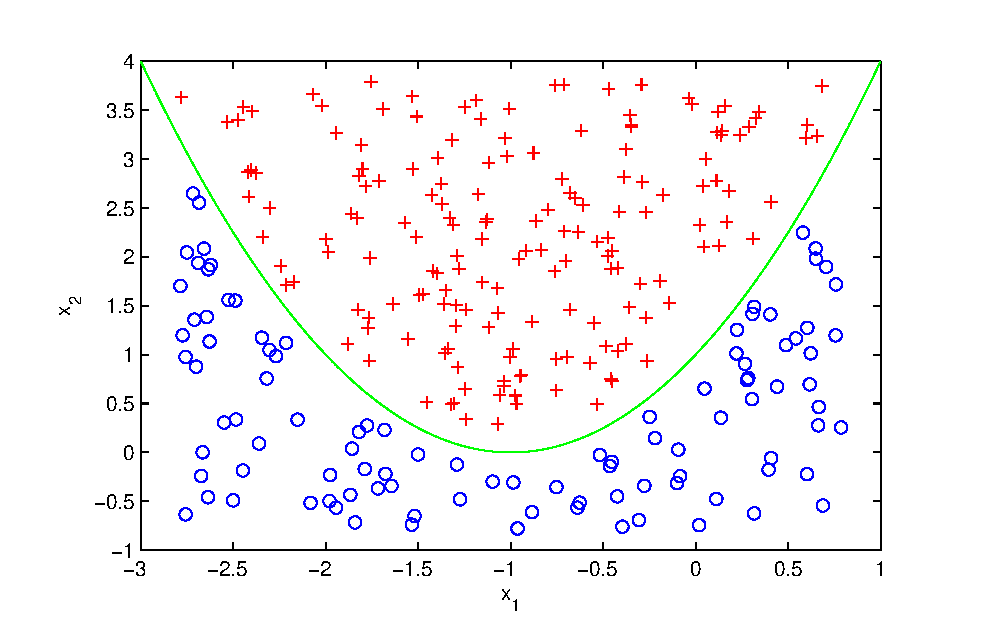
\includegraphics[width=0.50\textwidth]{images/fig21_featuresspace.eps}
\caption{
Configuration space vs. feature space. In this figure, the configuration space is $(x_1, x_2) \in \R^2$. The two classes are clearly separable by the green parabola, which is not linear. However, a linear binary classification model is able to separate the two classes as well using the (homogeneous) feature space $(1, x_1, x_1^2, x_2)$ and the weight vector $\w = (1, 2, 1, -1)$, both in $\R^4$.   
}
\label{fig:featuresspace}
\end{figure}


The goal of binary classification is to predict the class $\hat{t} \in \{ -1, 1 \}$ of a new observation $\x$. Linear binary classification achieves this by making a classification decision based on the value of a linear combination of the features. Specifically, the class prediction for $\x$ is based on the value of the following (so--called) predictor function \cite{bishop06}: 
\begin{equation} 
\label{eq:predictor}
f_{\w}(\x) = \sum_{j=1}^D w_j x_j + w_0 = \w^T \x + w_0,
\end{equation}
where $w_j$ is the weight corresponding to the $j-$th feature, $\w$ is the weight vector consisting of these individual weights, and $w_0$ is a bias (the negative of the bias is sometimes called a $threshold$). If $f_{\w}(\x) \geq 0$, the class prediction for $\x$ is $\hat{t} = 1$, otherwise $\hat{t} = -1$. Thus, the equation of the decision boundary that separates the two classes is $f_{\w}(\x) = \w^T \x + w_0 = 0,$
which is a hyperplane in this linear model (hence the decision boundary is also called \emph{decision hyperplane}). For convenience, the bias term is often included in the weight vector as $\begin{pmatrix}
w_0\\ \w \end{pmatrix}$, and the feature space is extended appropriately by a constant feature as $\begin{pmatrix} 1\\ \x \end{pmatrix}$. In this new notation, both $\w$ and $\x$ are in $\R^{D+1}$, and the predictor function is now $$f_{\w}(\x) = \w^T \x.$$ The equation of the decision hyperplane is now $$\w^T \x = 0,$$ which is a homogeneous system of equations. For this reason, this notation is called \emph{homogeneous}. For latter reference we call the former notation (with a separate bias $w_0$) \emph{non-homogeneous}. 

Note that the linear classification model may seem simple, but it can solve complicated problems as shown by Figure \ref{fig:featuresspace}, and is arguably the most commonly used classification model in practice. 

Clearly, to predict the class of a new observation, the weight vector $\w$ must have been already determined using a set of some ``historical'' observations with known class. In machine learning, this set is called the \emph{training dataset}, and contains some $N$ observations $\X = \{\boldsymbol{x_1, x_2, \dots, x_N}\}$ and their corresponding class $\t = \{t_1, t_2, \dots, t_N\}$. To measure the degree of belief in class prediction for an observation $\xi \in \X$, the so--called \emph{margin} is defined as follows:
\begin{equation} 
\label{eq:margin}
m_i(\w) = t_i f_{\w}(x_i),
\end{equation}
where $m_i(\w)$ is the margin corresponding to $\xi$. It can be seen that if $m_i(\w) < 0$ then the sign of the predictor function $f_{\w}(x_i)$ is opposite to the sign of then known class $t_i$ of point $\xi$, hence $\xi$ is misclassified. In this case, $m_i$ is a measure of the margin by which the class prediction for $\xi$ given by $f_{\w}(x_i)$ is wrong. Otherwise, if $m_i(\w) \geq 0$, then $\xi$ is correctly classified and $m_i$ represents the ``margin of safety'' by which the prediction is correct \cite{McAllester}.  

The task of classification is now boiled down to determine $\w$ based on the training dataset so as to minimize the sum of losses, where each loss quantifies the penalty for an incorrect classification in the training dataset. There are different types of losses used by different algorithms, such as 0--1 loss, log loss, squared loss, hinge loss, etc. Naturally, all these losses depend on the margin defined above, so the task is mathematically summarized as:
\begin{equation}
\label{eq:objective}
 \w^* = \arg\min_{\w} \; \sum_{i=1}^{N} L(m_i(\w)) + \lambda R(\w),
\end{equation}
where $L(m_i(\w))$ is some loss defined as a function of $m_i(\w)$, and the term $\lambda R(\w)$ is called the \emph{regularization term}, which prevents overfitting and extreme values of $\w$. In this term, $\lambda > 0$ is the \emph{regularization parameter}, which is tuned so as to maximize empirical performance of the resulting value of $\w^*$, and $R(\w)$ is the \emph{regularization function}, often defined as the $p-$norm of $\w$: 
$$R(\w) = \| \w \|_p = (\sum_{i=1}^D |w_i|^p)^{1/p}.$$
For instance, $p=1$ corresponds to the so--called $L_1$ regularizer: $$L_1(\w) = \sum_{i=1}^D |w_i|,$$ 
and $p=2$ corresponds to $L_2$ regularizer: $$L_2(\w) = \frac{1}{2} \w^T \w,$$ where the constant $\frac{1}{2}$ is added just for convenience, etc. 

We next review 0--1 loss and formulate the 0--1 loss optimization problem for linear binary classification. Other types of losses as well as their advantages and disadvantages shall be discussed in Section \ref{sec:bgr.surrogates}.   


%======================
\subsubsection{0--1 Loss and Problem Definition}
\label{ssec:01loss}

The 0--1 loss is defined for some margin $m$ as 
$$
L_{01}(m) = \left\{
     \begin{array}{ll}
       0 & : \text{if }m > 0\\
       1 & : \text{otherwise}
     \end{array}
   \right.
   \; = \; \mathbb{I} [m \leq 0],
$$
where the indicator function, $\mathbb{I} [.]$, is used to simplify the piecewise function. In the context of linear binary classification given in previous subsection, the margin is given by Equation \ref{eq:margin}, and the objective given by Equation \ref{eq:objective} now becomes
\begin{equation}
\label{eq:objective01}
 \w^* = \arg\min_{\w} \; \sum_{i=1}^{N} \mathbb{I} [t_i \w^T \xi \leq 0] + \lambda R(\w),
\end{equation}

It can be seen that in the context of 0--1 loss, the regularization term of the above objective function has no meaning as it can be always driven to zero by scaling down the weight vector $\w$ to $\epsilon \w$ with an arbitrarily small real positive constant $\epsilon$ without changing the 0--1 loss value, because the indicator function is invariant to such scaling. We can therefore omit this term, noting that in practice we can avoid overfitting by checking the components of $\w$ directly. The objective function now becomes
\begin{equation}
\label{eq:objective01}
 \w^* = \arg\min_{\w} \; \sum_{i=1}^{N} \mathbb{I} [t_i \w^T \xi \leq 0],
\end{equation}
where the sum of all losses $\sum_{i=1}^{N} \mathbb{I} [t_i \w^T \xi \leq 0]$ is called the 0--1 loss function. It can be seen, that the 0--1 loss function essentially counts the number of misclassifications. In this sense, 0--1 loss is the most natural loss function, because minimizing it is equivalent to minimizing the misclassification rate for the training data.

The subsequent chapters of this thesis study different approaches to optimize the 0--1 loss function. It is therefore convenient to give a unified problem definition for later reference as follows.

\begin{framed}
\label{definition}
{\bf The 0--1 Loss Optimization Problem Definition:}

\line(1,0){217}

Given a training dataset of $N$ observations $\X = \{\boldsymbol{x_1, x_2, \dots, x_N}\}$ and their corresponding targets $\t = \{t_1, t_2, \dots, t_N\}$, where  $\xi =  (1, x_{i1}, x_{i2}, \dots, x_{iD})^T \in \R^{D+1}$ and $t_i \in \{ -1, 1 \}$ for $i=1,2,\dots, N$. 

Find a weight vector $\w^*$, which minimizes the following 0--1 loss function:
\begin{equation}
\label{01loss}
L(\w) = \sum_{i=1}^N \mathbb{I} [t_i \w^T \xi \leq 0]
\end{equation}
where $\mathbb{I}$ is the indicator function, ${\w} = (w_0, w_1, \dots, w_D)^T \in \R^{D+1}$ is the (vector) variable of the 0--1 loss function $L(\w)$, and the task is to find (or approximate) 
$${\w}^* = \arg\min_{\w} L({\w})$$
\end{framed}

%=================================================
\subsection{Convex Optimization}
\label{sec:bgr.convexopt}

The objective function of the binary classification problem given by Equation \ref{eq:objective} is an optimization problem. Convex surrogates of 0--1 loss are often used in this objective function to gain computational efficiency. Thus, in this section we review gradient descent -- one of the first methods for convex optimization, keeping in mind that there are better methods like conjugate gradient, pseudo-Newton, etc., which are not in the scope of this thesis. A modified version of gradient descent called stochastic gradient descent is also reviewed. This version is suitable for situations where not all data are available at once. 

%======================
\subsubsection{Gradient Descent}

The convex optimization problem is defined as 
$$ \w^* = \arg \min_{\w} f(\w),$$
where $f(\w)$ is a convex function. 

The gradient descent method \cite{Cauchy} is based on the observation that if $f(\w)$ is defined and differentiable in a neighborhood of a point $\boldsymbol{a}$, then $f(\w)$ decreases fastest if one goes from $\boldsymbol{a}$ in the direction of the negative gradient of $f$ at $\boldsymbol{a}$, $-\nabla f(\boldsymbol{a})$. It follows that, if $\boldsymbol{b} = \boldsymbol{a} - \alpha \nabla f(\boldsymbol{a})$ for $\alpha \rightarrow 0$ a small enough number, then $f(\boldsymbol{a}) \geq f(\boldsymbol{b})$. With this observation in mind, the gradient descent method starts with a guess $\w^{(0)}$ and gradually updates it using 
$$\w^{(\tau + 1)} := \w^{(\tau)} - \alpha_{\tau} \nabla f(\w^{(\tau)}), $$
where $n \geq 0$, and the step size $\alpha_{\tau}$ is allowed to change in each step $\tau$. Then we have, 
$$f(\w^{(0)}) \geq f(\w^{(1)}) \geq f(\w^{(2)}) \geq \dots \;$$
Under the assumptions that $f(\w)$ is convex and $\nabla f(\w)$ Lipschitz, the sequence $(\w^{(\tau)})$ has been shown to converge to a local minimum, and because $f$ is convex, a local minimum is also global minimum. Thus, $(\w^{(\tau)})$ converges to the global solution $\w^*$.

%======================
\subsubsection{Stochastic Gradient Descent}
\label{ssec:sgd}

In machine learning, it often arises that the objective function is in the form
$$ \w^* = \arg \min_{\w} \sum_{i=1}^N f_i(\w),$$
where each function $f_i(.)$ is associated with the $i-$ observation of the training dataset. An example is the objective function for linear binary classification given by Equation \ref{eq:objective}. If the standard gradient descent is used to solve for $\w^*$, it is called \emph{batch learning}, and the update formula is 
$$\w^{(\tau +1)} := \w^{(\tau)} - \alpha \sum_{i=1}^N \nabla f_i(\w^{(\tau)}).$$

However, when the training dataset is big, the evaluation of the sum of gradients may become very expensive (due to limited availability of memory). In this case, stochastic gradient descent \cite{Davidon} is used to reduce the computational cost at every iteration, as it only samples a subset of summand functions' gradients. In this sense, it is also called \emph{online learning} or \emph{sequential learning}. In this case the update formula is 
$$\w^{(\tau +1)} := \w^{(\tau)} - \alpha \nabla f_i(\w^{(\tau)}).$$
We see that the individual gradient of an observation is used to approximate the sum of gradients. Often several passes over the training dataset are made until the algorithm converges. It has been shown by \cite{Bottou} and \cite{Kiwiel}, that when the learning rates decrease with an appropriate rate, and subject to relatively mild assumptions, stochastic gradient descent converges almost surely to a global minimum when the objective function is convex, and otherwise converges almost surely to a local minimum. 

%=================================================
\subsection{Surrogates of 0--1 Loss for Binary Classification}
\label{sec:bgr.surrogates}

In previous section we have reviewed the binary classification problem and 0--1 loss, minimizing which is equivalent to minimizing the error rate in the training dataset. However, direct optimization of 0--1 loss is NP--hard \cite{Feldman,nphard}, hence existing algorithms use convex surrogates of 0--1 loss. In this section, we first discuss the advantages and disadvantages of using a surrogate of 0--1 loss, and then review some of the most popular  surrogates and algorithms using them. Note that here we make heavy use of \cite{McAllester}, \cite{Webers}, \cite{bishop06}, and references therein.


%======================
\subsubsection{Advantages and Disadvantages of Surrogates}
\label{ssec:disadvantages}

Most state-of-the-art algorithms use some convex surrogate of 0--1 loss to solve the binary classification problem, because the convexity makes them computationally efficient \cite{Bartlett} and non-convexity often results in NP-hard problems. However, this choice comes at a cost as the disadvantages of convex objectives are well understood. Intuitively, loss should be bounded as we should not pay an infinite cost for misclassifying any one observation. It can be seen in Figure \ref{fig:losses}, that 0--1 loss is bounded, while other convex surrogates are not bounded with large negative margins. Because of this reason, \cite{outliers} showed that convex loss functions cannot be made robust in the presence of  noise. \cite{outliers2} further characterized this effect by analyzing various convex losses and found that risk minimization under 0-1 loss function has impressive noise tolerance properties and that under squared error loss is tolerant only to uniform noise; risk minimization under other loss functions is not noise tolerant.

%======================
\subsubsection{Squared Loss and Linear Regression}

The squared loss is defined as follows:

\[ \begin{split}
L_2(m_i(\w)) &= \frac{1}{2}[m_i(\w) - 1]^2 \\
& = \frac{1}{2}[t_i f_{\w}(\xi) - t_i^2]^2 \\
& = \frac{1}{2}t_i^2 [f_{\w}(\xi) - t_i]^2 \\
& = \frac{1}{2}[\w^T\xi - t_i]^2,
\end{split} \] 
where we used the fact that $t_i^2 = 1$, and the constant $\frac{1}{2}$ is used for later convenience. We see that minimizing (the sum of) squared loss is equivalent to minimizing the (total squared) difference between the value given by the predictor function $\w^T\xi$ and the training target $t_i$. By applying this loss to the objective function of binary classification given by Equation \ref{eq:objective01} we have the following:
\begin{equation}
\label{eq:squareobj}
\w^* = \arg\min_{\w} \; \sum_{i=1}^{N}  \frac{1}{2}[\w^T\xi - t_i]^2 + \lambda R(\w).
\end{equation}
Squared loss is often used with $L_2$ or $L_1$ regularizers. It is called \emph{ridge regression} if used with $L_2$ regularizer, or \emph{lasso} if used with $L_1$. We further consider ridge regression (keeping in mind that lasso is similar), in this case the objective function becomes 
\[ \begin{split}
\w^* & = \arg\min_{\w} \;  \frac{1}{2} \sum_{i=1}^{N} [\w^T\xi - t_i]^2 + \frac{\lambda}{2} \w^T\w \\
& = \arg\min_{\w} \; \{  \frac{1}{2}(\t - \X\w)^T(\t - \X\w) + \frac{\lambda}{2} \w^T\w \},
\end{split} \]
where 
$\t = \begin{pmatrix} t_1\\ t_2 \\ \vdots \\ t_N \end{pmatrix}$, and 
$\X = \begin{pmatrix} \boldsymbol{x_1}\\ \boldsymbol{x_2}\\ \vdots \\ \boldsymbol{x_N}\end{pmatrix}$. 
Let $g(\w)$ denote the function to be optimized: 
$$ g(\w) = \frac{1}{2}(\t - \X\w)^T(\t - \X\w) + \frac{\lambda}{2} \w^T\w.$$
This is a convex function and there are two ways to optimize it: analytical and sequential, both are addressed as follows.

For the \emph{analytical solution}, we calculate the gradient of $g(\w)$ and set it to zero: 
\[ \begin{split}
& \nabla g(\w) = \X^T(\X\w - \t) + \lambda\w = \boldsymbol{0}  \\
\Leftrightarrow \quad & (\X^T \X + \lambda \boldsymbol{I}) \w = \X^T \t \\
\Leftrightarrow \quad & \w^* = (\X^T\X + \lambda \boldsymbol{I})^{-1}\X^T \t, 
\end{split} \]
where $\boldsymbol{I}$ denotes the identity matrix. It is easy to check that the Hessian matrix $$H(g) = \X^T\X + \lambda \boldsymbol{I}$$ is positive semi definite, so $\w^*$ is a local minimum. As $g(\w)$ is convex, $\w^*$ is also the global minimum. Thus, $\w^* = (\X^T\X + \lambda \boldsymbol{I})^{-1}\X^T \t$ is the \emph{closed form solution} to the objective function given by Equation \ref{eq:squareobj}.

For big datasets, however, the calculation of the given closed form solution of $\w^*$ may be very expensive. In this case, the \emph{online learning} approach is used by applying the stochastic gradient descent method discussed in Subsection \ref{ssec:sgd}. The concrete \emph{linear regression} procedure is given as follows. 
\begin{description}
\setlength{\itemsep}{0cm}
\setlength{\parskip}{0cm}
\item[Step 1:] \hfill \\initialize $\w$ to some initial value
\item[Step 2:] \hfill \\update $\w$ in each iteration by: 
$$\w := \w - \alpha (\nabla L(m_i(\w)) + \lambda \w)$$
\end{description}
where $\nabla L(m_i(\w))$ is the gradient of an individual loss, in this case the squared loss of the $i-$th point:
$$\nabla L(m_i(\w)) = (\w^T \xi - t_i)\xi,$$
and the step size $\alpha$ (also called \emph{learning rate}) must be chosen carefully, as a too large learning rate prevents algorithm from converging and a too small learning rate updates $\w$ too slowly. Often several passes over the training set are made until the algorithm converges. Typical implementations may also randomly shuffle training examples at each pass and use an adaptive learning rate.

%======================
\subsubsection{Log Loss and Logistic Regression}

We have discussed in Subsection \ref{ssec:binclass}, that if $m_i < 0$ then $|m_i|$ is a measure of the margin by which the class prediction for $\xi$ given by $f_{\w}(x_i)$ is wrong, otherwise the prediction is correct. In this sense, the log loss is defined as 
\[ \begin{split}
L_{log}(m_i(\w)) &= \ln (1 + e^{-m_i(\w)}) \\
 &= \ln (1 + e^{-t_i\w^T\xi}) 
\end{split} \] 
It can be easily verified, that this loss is convex, and for $m_i >> 1$ we have $L_{log}(m_i) \approx 0$, on the other hand, for $m_i << -1$ we have $L_{log} \approx -m_i = |m_i|$. In other words, log loss is a convex model of the scheme, where misclassification is penalized by the absolute value of the margin, and correct classification has zero penalty. We note that both log loss and quadratic loss can be viewed as an attempt to estimate $P(t|\x)$ and can be derived under assumption that $P(\x|t)$ has (multivariate) Gaussian distribution. However, for the purpose here we will not go into this detail. By applying log loss to the objective function of binary classification given by Equation \ref{eq:objective01} we have the following:
\begin{equation}
\label{eq:logobj}
\w^* = \arg\min_{\w} \; \sum_{i=1}^{N} \ln(1 + e^{-t_i\w^T\xi})  + \lambda R(\w).
\end{equation}

\emph{Logistic regression} is the combination of log loss with $L_2$ regularizer, where the objective function becomes 
\[ \begin{split}
\w^* & = \arg\min_{\w} \; \sum_{i=1}^{N} \ln(1 + e^{-t_i\w^T\xi}) + \frac{\lambda}{2} \w^T\w \\
\end{split} \]

In contrast to the previous case, this time there is no closed form solution for $\w^*$. So we have to revert to an iterative procedure, e.g., batch learning or online learning discussed in Subsection \ref{ssec:sgd}. A concrete regression procedure has been given in the previous subsection. Here for completeness, we will derive the update form. Let $g(\w)$ denote the function to be optimized:
$$ g(\w) = \sum_{i=1}^{N} \ln(1 + e^{-t_i\w^T\xi}) + \frac{\lambda}{2} \w^T\w.$$
Then its gradient is 
\[ \begin{split}
 \nabla g(\w) &= \sum_{i=1}^{N} \frac{1}{1+e^{-t_i \w^T \xi}}e^{-t_i \w^T \xi} (-t_i \xi) + \lambda \w \\
 &= - \sum_{i=1}^{N} \frac{1}{1 + e^{t_i \w^T \xi}} t_i \xi + \lambda \w \\
 &= - \sum_{i=1}^{N} \sigma(-m_i(\w)) \, t_i \xi + \lambda \w,
\end{split} \]
where $\sigma(a) = \frac{1}{1 + exp(-a)}$ is called the logistic sigmoid function. With the gradient available, it is now easy to derive the update form. For batch learning it is
$$\w := \w + \alpha \sum_{i=1}^{N} \sigma(-m_i(\w)) \, t_i \xi - \alpha \lambda \w.$$
And for online learning it is
$$\w := \w + \alpha \, \sigma(-m_i(\w)) \, t_i \xi - \alpha \lambda \w.$$
Note that for a same training dataset, the regularization constant $\lambda$ for online learning would be much smaller than that for batch learning. 


%======================
\subsubsection{Hinge Loss and Support Vector Machine}

The hinge loss is defined as
\[ \begin{split}
L_{hinge}(m_i(\w)) &= \max(0, 1 - m_i(\w)) \\
&= \max(0, 1 - t_i \w^T \xi),
\end{split} \] 
and it can be viewed as a piecewise linear approximation of log loss, because it has the same properties as given for log loss for cases when $m_i >> 1$ and $m_i << -1$. Although being convex, this loss is difficult to optimize directly using the traditional procedure. To be more specific, applying this loss with $L_2$ regularizer to Equation \ref{eq:objective} yields 
\begin{equation}
\label{eq:svmobj}
\w^* = \arg\min_{\w} \; \sum_{i=1}^{N} \max(0,1 - t_i\w^T\xi)  + \frac{\lambda}{2} \w^T\w,
\end{equation}
which is non--differentiable, so typical optimization methods cannot be directly applied. However, the support vector machines (SVM) method proposed by \cite{Vapnik} minimizes this loss by using the maximum-margin classification approach, which we briefly review the key points of this method as follows.

First, suppose that the two classes of the discussed linear binary classification problem are linearly separable by some weight vector $\w$. Then, SVM chooses the decision boundary which maximizes the smallest distance to samples in both classes, which is mathematically defined as
$$ \w^* = \arg \max_{\w} \{ \frac{1}{\|\w\|} \min_i [t_i\w^T \xi] \}. $$
We have discussed in Subsection \ref{ssec:01loss}, that scaling $\w$ to $\epsilon \w$ does not change the decision hyperplane. Thus we can scale $\w$ in such a way that for the closest point $t_i\w^T \xi = 1$. Then the objective function becomes 
\[ \begin{split}
& \w^* = \arg \max_{\w} \{ \frac{1}{\|\w\|} \} \quad s.t. \quad \;t_i\w^T \xi \geq 1 \quad \forall i = 1, 2, \dots, N \\
\Leftrightarrow \quad &  \w^* = \arg \min_{\w} \{ \frac{1}{2}\|\w\|^2 \} \quad s.t. \quad \;t_i\w^T \xi \geq 1 \quad \forall i = 1, 2, \dots, N.
\end{split} \] 
This is a quadratic programming problem: minimize a quadratic function subject to linear constraints, and can be efficiently solved using the method of Lagrange multipliers with the Karush�Kuhn�Tucker (KKT) conditions \cite{Kuhn}. 

Now, for the case when the two classes are not linearly separable, hinge loss is used to penalize data points that are on the `wrong side' of the decision boundary as follows:
$$L_{hinge}(m_i) 
\left\{
     \begin{array}{ll}
       = 0 & : \xi \text{ is correctly classified and on or beyond the margin}\\
       < 1 & : \xi \text{ is in the correct margin}\\
       = 1 & : \xi \text{ is on the decision boundary}\\
       > 1 & : \xi \text{ is misclassified, penalty } \approx |m_i|
     \end{array}
   \right..
$$
The constraints are now changed to 
$$ t_i\w^T \xi \geq 1 - L_{hinge}(m_i) \quad \forall i = 1, 2, \dots, N,$$
and the objective is to minimize 
$$ C \sum_{i=1}^N L_{hinge}(m_i) + \frac{1}{2} \w^T\w,$$  
where the constant $C$ controls the trade-off between the loss and the margin. To sum up, the full objective function is:
\[ \begin{split}
\w^* = \arg\min_{\w} \{ C \sum_{i=1}^N  \max(0, 1 - t_i \w^T \xi) + \frac{1}{2} \w^T\w \} \\
s.t. \quad t_i\w^T \xi \geq 1 - \max(0, 1 - t_i \w^T \xi) \quad \forall i = 1, 2, \dots, N.
\end{split} \] 
We see that this is, again, a quadratic programming problem, which can be solved efficiently as discussed before. Furthermore, this function is similar to the objective function given by Equation \ref{eq:svmobj}, with the only difference in the constants $\lambda$ and $C$, both of them, however, can be treated as a regularization constant.


%=================================================
\subsection{Other Methods for Binary Classification}
\label{sec:bgr.others}

In the previous section, we have reviewed some of the most popular methods for binary classification. In this section, we will briefly review some other methods that have not been mentioned. The first subsection is devoted to Bayes point machine. The subsequent subsection then summarizes several other methods.  

%======================
\subsubsection{Bayes Point Machine}

Bayes point machine (BPM) was proposed by \cite{Herbrich}. This is a Bayesian approach to linear classification and is briefly summarized as follows. From our discussion in Subsection \ref{ssec:binclass} we see that, in linear classification, a point $\x$ is classified by $t = \sign(\w^T \x)$ for some weight vector $\w$. Given the training dataset $\D = \{\X, \t \}$, the likelihood for $\w$ is given by
$$p(\D | \w) = \prod_{i=1}^N p(t_i | \xi, \w) = \prod_{i=1}^N \phi(\frac{t_i\w^T\xi}{\epsilon}),$$
where 
$$\phi(z) = \int_{-\infty}^z N(z; 0, 1) dz,$$
and $\epsilon$ controls the allowed `slack'. By using $\phi$ instead of a step function, this likelihood tolerates small errors. Under the Bayesian approach, we also have a prior distribution of $\w$, which is taken to be the zero-mean unit-variance normal distribution: $N(\boldsymbol{0, I})$. Given this model, the optimal way to classify a new data point $\x$ is to vote all classifiers according to their posterior probability: $\mathbb{E}[\sign(\w^T \x) | \D]$. This is, however, expensive to compute. As an approximation to this, BPM uses the output of the average classifier: $\sign(\mathbb{E}[\w] ^T \x)$. This can be estimated by the billiard ball algorithm proposed in the original BPM paper, which is based on the Monte Carlo method. Another (better) way to estimate this is by using expectation propagation as proposed by \cite{bpm}. This thesis uses the Matlab implementation of expectation propagation algorithm for BPM of the latter author in all comparisons where BPM is present. 

%======================
\subsubsection{Other Methods}

Apart from mentioned algorithms, there are quite a few other algorithms that can solve the binary classification problem. Some of the most notable are, for example, the following. Neural networks \cite{bishop2} consist of one or more interconnected layers of neurons, each neuron having its own weight vector. It can be viewed as an adaptive system that changes its structure during learning phase. In contrast to the introduced linear binary classification model, neural networks is generally not linear, except for perceptrons \cite{perceptron}, which can be considered as the simplest kind of neural network. Perceptron, however, may not converge if the two classes are not linearly separable. $k-$ Nearest Neighbor \cite{kNN} is one of the simplest classification algorithms. It assigns a new data point to the class most common amongst its $k$ nearest training data points (neighbors). Adaboost \cite{adaboost}, short for Adaptive Boosting, is an algorithm that coordinate several weak classifiers to improve the classification quality, where subsequent classifiers are tweaked in favor of those instances misclassified by previous classifiers. Adaboost uses exponential loss, which is $L_{exp} = \exp(-m_i(\w)) = \exp(-t_i\w^T\xi)$, hence can be sensitive to noisy data and outliers. Decision trees are also used for classification as shown by \cite{tree1}, and by \cite{tree2}. 

There are also many works that are more or less related to the work of this thesis. We can categorize them into those developing classifiers that are robust to outliers and those optimizing 0--1 loss directly. The number of works in the first category is quite abundant, including t-logistic regression \cite{Ding}, robust truncated hinge loss \cite{robusthinge}, SavageBoost \cite{lossdesign}, and more. There are, however, almost no works in the second category. At the time of finishing this thesis, we can only find the work by \cite{ling}, which proposes an algorithm optimizing 0--1 loss for perceptrons by random coordinate descent. 


%=================================================
\subsection{Summary}
\label{sec:bgr.summary}

In this chapter, we have reviewed the linear binary classification problem and several popular methods for it. However, these methods depend on convex surrogates of 0--1 loss, hence suffer from the presence of noise and outliers in the training set as discussed in Subsection \ref{ssec:disadvantages}. One strategy to avoid this problem is to optimize 0-1 loss directly, and this is the topic of study in the remaining chapters of the thesis. 

%%% Local Variables: 
%%% mode: latex
%%% TeX-master: "thesis"
%%% End: 

    \section{Parameterized Hybrid MDPs}
\label{sec:hybrid_mdps}

In this Section we introduce parameterized hybrid Markov Decision Processes (PHMDPs) and show how the framework can be specialized to investigate multi-objective rewards, parameter sensitivity and non-convex optimization of policy parameters. We also review their finite horizon solution via dynamic programming.

\subsection{Definition}
\label{sec:hybrid_mdps_def}

A parameterized hybrid Markov Decision Process (PHMDP) is defined by the tuple {\footnotesize \PMDPTuple}. {\footnotesize \State} specifies a vector of states given by {\footnotesize $(\vec{d}, \vec{x}) = \left( d_1, \ldots, d_m, x_1, \ldots, x_n \right) $}, where each {\footnotesize $ d_i \in \left\lbrace 0, 1 \right\rbrace $} {\footnotesize $\left( 1 \leq i \leq m \right)$} is boolean and each {\footnotesize$ x_j \in \Real $} {\footnotesize $\left( 1 \leq j \leq n \right)$} is continuous. {\footnotesize \Action} specifies a finite set of actions. PHMDPs
are naturally factored~\parencite{Boutilier_JAIR_1999} in terms of the state variables {\footnotesize$\vec{d}$, $\vec{x}$} and as such, the joint transition model can be written as:
{\footnotesize
\abovedisplayskip=0pt
\belowdisplayskip=0pt
\begin{align}
    \label{eq:hmdp_tfunc}
    \Transition :& \, \ProbArg{\vec{d}', \vec{x}' | \vec{d}, \vec{x}, a, \theta} = \nonumber \\
    & \prod_{i=1}^{m} \ProbArg{d_i' | \vec{d}, \vec{x}, a, \theta} \prod_{j=1}^{n} \ProbArg{x_j' | \vec{d}, \vec{d}', \vec{x}, a, \theta}.
\end{align}   
}

{\footnotesize \RewardFunc} is the reward function which encodes the preferences of the agent. {\footnotesize \Horizon} represents the number of decision steps until termination and the discount factor {\footnotesize $\gamma \in [0, 1)$} is used to geometrically discount future rewards. {\footnotesize $\theta \in \Theta$} is a free parameter from the parameter space {\footnotesize $ \Theta $}.

A policy {\footnotesize $\pi : \State \rightarrow \Action$}, specifies the action to take in every state. The value of a state {\footnotesize $(\vec{d}, \vec{x}) \in \State$} under a given policy {\footnotesize$\pi$} is given by:
{\footnotesize 
    \abovedisplayskip=0pt
    \belowdisplayskip=0pt
\begin{align*}
    V^{\pi}\left( \vec{d}, \vec{x}; \theta \right) &= \Exp{\sum\limits_{h = 0}^{\Horizon} \gamma^h \cdot r^h | \vec{d}, \vec{x}, \theta} \nonumber  
%    &= \sum\limits_{s' \in \State}  \Transition\left(s, \pi\left(s\right), s' \right) \left[ \Reward\left(s, \pi(s), s'\right) + \gamma \cdot V^{\pi}(s')\right]. \label{eq:mdp_bellman_eq}
\end{align*}
}
%Equation~\eqref{eq:mdp_bellman_eq} is known as the Bellman equation for $V^{\pi}$.

The state-action value function {\footnotesize$Q : \State \times \Action \rightarrow \mathbb{R}$} is given by:
{\footnotesize 
    \abovedisplayskip=0pt
    \belowdisplayskip=0pt
\begin{align*}
%    \label{eq:mdp_qfunc}
    Q^{\pi}\left(\vec{d}, \vec{x}, a; \theta\right) = \Exp{\sum\limits_{h = 0}^{\Horizon} \gamma^h \cdot r^h | \vec{d}, \vec{x}, a, \theta}.
\end{align*}
}

The optimal value function of policy {\footnotesize$ \pi^{*} $} satisfies
{\footnotesize 
\abovedisplayskip=0pt
\belowdisplayskip=0pt
\begin{align}
    \label{eq:opt_vfunc}
    V^{\pi^{*}}(\vec{d}, \vec{x}; \theta) &= \max_{a \in A} \left\{ Q^{\pi^{*}}(\vec{d}, \vec{x}, a; \theta) \right\}. 
\end{align}
}%

We note that in our formulation of parameterized hybrid MDPs the parameters {\footnotesize $ \theta $} are not learned, which is in contrast to the work of~\parencite{Dearden_UAI_1999}.

In the subsequent Sections we demonstrate how the PHMDP framework can be specialised into models capable of: (i) investigating multi-objective trade-offs; (ii) exact sensitivity analysis; and (iii) non-convex optimization of policy parameters.

\subsubsection{Multi-objective PHMDPs}

The PHMDP framework can be specialised into a multi-objective setting by specifying the reward as {\footnotesize \MORewardFunc} where {\footnotesize $ d $} is the dimension of the reward vector. In this formulation the parameter {\footnotesize $ \theta^{d} $}, specifies the preferences over the reward components.

\subsubsection{Sensitivity Analysis for PHMDPs}

Sensitivity analysis can be conducted within the PHMDP framework by specifying as value function as in Equation~\eqref{eq:opt_vfunc}. The value function can then be differentiated with respect to the parameter {\footnotesize $ \theta $}.

\subsubsection{Policy Gradient Methods for PHMDPs}

PHMDP policy parameters can be optimised by specifying the action {\footnotesize \Action} as {\footnotesize $ a(\theta) $}.

\subsection{Solution Methods}

Value iteration~\parencite{Bellman_PU_1957} is a general dynamic programming algorithm used to solve MDPs. We modify the algorithm to solve the parameterized hybrid MDP formulation presented in Section~\ref{sec:hybrid_mdps_def}. The key idea of VI is to successively approximate {\footnotesize $V^{\pi^{*}}(\vec{d}, \vec{x}; \theta)$} and {\footnotesize $Q^{\pi^{*}}(\vec{d}, \vec{x}, a; \theta)$} by {\footnotesize $V^{h}(\vec{d}, \vec{x}; \theta)$} and {\footnotesize $Q^{h}(\vec{d}, \vec{x}, a; \theta)$}, respectively, at each horizon {\footnotesize$h$}. These two functions satisfy the following recursive relationship:

{\footnotesize 
    \abovedisplayskip=0pt
    \belowdisplayskip=0pt
    \begin{align}
        Q^{h}(\vec{d}, \vec{x}, a; \theta) &= \Reward(\vec{d}, \vec{x}, a; \theta) + \gamma \cdot  \nonumber \\ 
        & \sum_{\vec{d}'} \int_{\vec{x}'} \ProbArg{\vec{d}', \vec{x}' | \vec{d}, \vec{x}, a; \theta} \cdot V^{h-1}(\vec{d}, \vec{x}; \theta) d\vec{x}' \label{eq:vi_qfunc} \\
        V^{h}(\vec{d}, \vec{x}; \theta) &= \max_{a \in A} \left\{ Q^{h}(\vec{d}, \vec{x}, a; \theta) \right\} \label{eq:vi_vfunc}
    \end{align}
}%

The algorithm can be executed by first initialising {\footnotesize $V^{0}(\vec{d}, \vec{x}; \theta)$}  to zero or the terminal reward. Then for each {\footnotesize$h$}, {\footnotesize $V^{h}(\vec{d}, \vec{x}; \theta)$} is calculated from {\footnotesize $V^{h-1}(\vec{d}, \vec{x}; \theta)$} via Equations~\eqref{eq:vi_qfunc} and~\eqref{eq:vi_vfunc}, until the intended $h$-stage-to-go value function is computed. 

%Value iteration converges linearly in the number of iterations to the true values of {\footnotesize $Q^{\pi^{*}}(\vec{d}, \vec{x}, a; \theta)$} and {\footnotesize $V^{\pi^{*}}(\vec{d}, \vec{x}; \theta)$}~\parencite{Bertsekas_1987}.

%One key challenge still remains, namely, dealing with the infinitely
%many states in $\vec{x}$. We know that the {\footnotesize $V^{h}(\vec{x})$} and 
%{\footnotesize $Q^{h}(\vec{x}, a_1, a_2)$} functions have structure, but are unable to derive
%them. Furthermore, given known structures for {\footnotesize $V^{h}(\vec{x})$} and 
%{\footnotesize $Q^{h}(\vec{x}, a_1, a_2)$} we must determine the restrictions that
%guarantee a tractable solution. The SDP framework in conjunction with its
%closed-form operations provide answers to both of these concerns.

In the next section we show that parameterized hybrid MDPs can be solved optimally for arbitrary horizons using symbolic dynamic programming.
    In order to compute the equations above, we propose a \emph{Robust symbolic dynamic programming} approach similar to ~\cite{sanner_uai11}.  This requires a general value iteration in Algorithm~\ref{alg:vi} (\texttt{VI})
and a regression subroutine in Algorithm~\ref{alg:regress}
(\texttt{Regress}) %where we have omitted parameters $\vec{b}$ and $\vec{x}$ from $V$ and $Q$ to avoid notational clutter. 
%Note that the noise variables are defined and minimized in the 
%Before we explain this contribution though, we ~\ref{alg:vi} Algorithm. 
In general Symbolic Dynamic Programming (SDP) uses the \emph{case} representation. All operations required for computing $Q$ and $V$ functions are \emph{case operations} and defined next. We then move to the Robust SDP solution. 

\subsection{Case Representation and Operators}

Symbolic functions can generally be represented in \emph{case} form~\cite{fomdp}:
{%\footnotesize 
\begin{align}
f = 
\begin{cases}
  \phi_1: & f_1 \\ 
 \vdots&\vdots\\ 
  \phi_k: & f_k \\ 
\end{cases} \label{eq:case}
\end{align}
}
where $\phi_i$ are logical formulae defined over the state
$(\vec{b},\vec{x})$ and can include arbitrary logical ($\land,\lor,\neg$)
combinations of boolean variables and \emph{linear} inequalities ($\geq,>,\leq,<$) 
over continuous variables.  
%Each $\phi_i$ will be disjoint from the other $\phi_j$ ($j \neq i$);  however the $\phi_i$ may not exhaustively cover the state space, hence $f$ may only be a \emph{partial function} and may be undefined for some variable assignments.

The $f_i$ may be either linear or quadratic in the continuous parameters according to the same restrictions as for 
$R(\vec{b},\vec{x},a,\vec{y})$and to be continuous at partition boundaries. 


%%%%%%%%%%%%%%%%%%%%%%%%%%%%%%%%%%%%%%%%%%%%%%%%%%%%%%%%%%%%%%%%%%%%%%%%
\incmargin{.5em}
\linesnumbered
\begin{algorithm}[t!]
\vspace{-.5mm}
\dontprintsemicolon
\SetKwFunction{regress}{Regress}
\Begin{
   $V^0:=0, h:=0$\;
   \While{$h < H$}{
       $h:=h+1$\;
       \ForEach {$a(\vec{y}) \in A$}{
              $Q_a^{h}(\vec{y})\,:=\,$\regress{$V^{h-1},a,\vec{y}$}\;
               $Q_a^{h}(\vec{y},\vec{\epsilon}) := \casemax_{\vec{epsilon}} \, Q_a^{h}(\vec{y})$ $\,$ \emph{// $\max$-in noise variables}\;
				$Q_a^{h}(\vec{y}) := \min_{\vec{epsilon}} \, Q_a^{h}(\vec{y},\vec{\epsilon})$ $\,$ \emph{// Stochastic $\min$}\;
				$Q_a^{h} := \max_{\vec{y}} \, Q_a^{h}(\vec{y})$ $\,$ \emph{// Continuous $\max$}\;
              $V^{h} := \casemax_a \, Q_a^{h}$ $\,$ \emph{// $\casemax$ all $Q_a$}\;
              $\pi^{*,h} := \argmax_{(a,\vec{y})} \, Q_a^{h}(\vec{y})$\;
       }
       \If{$V^h = V^{h-1}$}
           {break $\,$ \emph{// Terminate if early convergence}\;}
   }
     \Return{$(V^h,\pi^{*,h})$} \;
}
\caption{\footnotesize \texttt{VI}(CSA-MDP, $H$) $\longrightarrow$ $(V^h,\pi^{*,h})$ \label{alg:vi}}
\vspace{-1mm}
\end{algorithm}
\decmargin{.5em}
%%%%%%%%%%%%%%%%%%%%%%%%%%%%%%%%%%%%%%%%%%%%%%%%%%%%%%%%%%%%%%%%%

%%%%%%%%%%%%%%%%%%%%%%%%%%%%%%%%%%%%%%%%%%%%%%%%%%%%%%%%%%%%%%%%%
\incmargin{.5em}
\linesnumbered
\begin{algorithm}[t!]
\vspace{-.5mm}
\dontprintsemicolon
\SetKwFunction{remapWithPrimes}{Prime}
%\SetKwFunction{sumout}{sumout}


\Begin{
    $Q=$ \remapWithPrimes{$V$} $\,$ \emph{// All $b_i \to b_i'$ and all $ x_i \to x_i'$} \;
    \emph{// Continuous regression marginal integration}\\
    \For {all $x'_j$ in $Q$}{
         $Q := \int Q \otimes P(x_j'|\vec{b},\vec{b}',\vec{x},a,\vec{y},\vec{\epsilon}) \, d_{x'_j}$\;
    }
    \emph{// Discrete regression marginal summation}\\
    \For {all $b'_i$ in $Q$}{
         $Q := \left[ Q \otimes P(b_i'|\vec{b},\vec{x},a,\vec{y}) \right]|_{b_i' = 1}$\\
         \hspace{8mm} $\oplus \left[ Q \otimes P(b_i'|\vec{b},\vec{x},a,\vec{y}) \right]|_{b_i' = 0}$\;
    }
    \Return{$R(\vec{b},\vec{x},a,\vec{y}) \oplus (\gamma \otimes Q)$} \;
}
\caption{\footnotesize \texttt{Regress}($V,a,\vec{y}$) $\longrightarrow$ $Q$ \label{alg:regress}}
\vspace{-1mm}
\end{algorithm}
\decmargin{.5em}
%%%%%%%%%%%%%%%%%%%%%%%%%%%%%%%%%%%%%%%%%%%%%%%%%%%%%%%%%%%%%%%%%

For any \emph{Unary operations} such as scalar multiplication $c\cdot f$ (for
a constant $c \in \mathbb{R}$) and negation $-f$ on case statements
$f$, the operation is simply applied to each
$f_i$ ($1 \leq i \leq k$). \emph{Binary operation} on two case statementsare done by taking the cross-product
of the logical partitions of the two case statement and perform the
corresponding operation on the resulting paired partitions.  As a  example the ``cross-sum'' $\oplus$ of two cases are defined as below

{\footnotesize 
\begin{center}
\begin{tabular}{r c c c l}
&
\hspace{-6mm} 
  $\begin{cases}
    \phi_1: & f_1 \\ 
    \phi_2: & f_2 \\ 
  \end{cases}$
$\oplus$
&
\hspace{-4mm}
  $\begin{cases}
    \psi_1: & g_1 \\ 
    \psi_2: & g_2 \\ 
  \end{cases}$
&
\hspace{-2mm} 
$ = $
&
\hspace{-2mm}
  $\begin{cases}
  \phi_1 \wedge \psi_1: & f_1 + g_1 \\ 
  \phi_1 \wedge \psi_2: & f_1 + g_2 \\ 
  \phi_2 \wedge \psi_1: & f_2 + g_1 \\ 
  \phi_2 \wedge \psi_2: & f_2 + g_2 \\ 
  \end{cases}$
\end{tabular}
\end{center}
}
\normalsize

The other operations of $\ominus$ and $\otimes$ are performed by subtracting or multiplying partition values.  Note that some partitions may become inconsistent (infeasible)  which are removed from the final result. 

The other operations required for RSDP are restriction, substitution and maximization on case statements.  

\texttt{Regression} is defined separately for discrete and continuous variables.\emph{Boolean restriction} $f|_{b=v}$ assigns the value $v \in \{ 0,1 \}$ to any occurrence of $b$ in $f$ such as lines 7--8. \emph{Continuous integration} $\int Q(x'_j) \otimes P(x'_j|\cdots) dx'_j$  us performed in line 5 where $P(x_j'|\cdots)$
is in the form of $\delta[x_j' - h(\vec{z})]$ ($h(\vec{z})$ is a case statement and $\vec{z}$ does not contain
$x'_j$) and the result from integration is $\int f(x'_j) \otimes \delta[x_j' - h(\vec{z})] dx'_j = f(x'_j) \{ x'_j / h(\vec{z}) \}$. Note that the latter operation indicates that any occurrence of $x'_j$ in
$f(x'_j)$ is \emph{symbolically substituted} with the case statement
$h(\vec{z})$.  Full specification of this operation is defined in~\cite{sanner_uai11}. 
A \emph{symbolic case maximization} on two case statements is performed below:
\vspace{-4mm}

{\footnotesize
\begin{center}
\begin{tabular}{r c c c l}
&
\hspace{-7mm} $\casemax \Bigg(
  \begin{cases}
    \phi_1: \hspace{-2mm} & \hspace{-2mm} f_1 \\ 
    \phi_2: \hspace{-2mm} & \hspace{-2mm} f_2 \\ 
  \end{cases}$
$,$
&
\hspace{-4mm}
  $\begin{cases}
    \psi_1: \hspace{-2mm} & \hspace{-2mm} g_1 \\ 
    \psi_2: \hspace{-2mm} & \hspace{-2mm} g_2 \\ 
  \end{cases} \Bigg)$
&
\hspace{-4mm} 
$ = $
&
\hspace{-4mm}
  $\begin{cases}
  \phi_1 \wedge \psi_1 \wedge f_1 > g_1    : & \hspace{-2mm} f_1 \\ 
  \phi_1 \wedge \psi_1 \wedge f_1 \leq g_1 : & \hspace{-2mm} g_1 \\ 
  \phi_1 \wedge \psi_2 \wedge f_1 > g_2    : & \hspace{-2mm}f_1 \\ 
  \phi_1 \wedge \psi_2 \wedge f_1 \leq g_2 : & \hspace{-2mm} g_2 \\ 
 % \vdots & \vdots
 \phi_2 \wedge \psi_1 \wedge f_2 > g_1    : & \hspace{-2mm} f_2 \\ 
 \phi_2 \wedge \psi_1 \wedge f_2 \leq g_1 : & \hspace{-2mm} g_1 \\ 
 \phi_2 \wedge \psi_2 \wedge f_2 > g_2    : & \hspace{-2mm} f_2 \\ 
 \phi_2 \wedge \psi_2 \wedge f_2 \leq g_2 : & \hspace{-2mm} g_2 \\ 
  \end{cases}$
\end{tabular}
\end{center}
} If all $f_i$ and $g_i$ are linear,
the $\casemax$ result is clearly still linear.  If the $f_i$ or $g_i$
are quadratic (e.g. in the reward), then $f_i > g_i$ or $f_i \leq
g_i$ will be at most univariate quadratic which can be linearized into two linear inequalities. Hence the result of this $\casemax$
operator will be representable in the case format with linear inequalities in decisions.

For continuous maximization according to ~\cite{sdp_aaai} the $\max_y$ for each case partition
is computed individually that is $\max_y \phi_i(\vec{b},\vec{x},y) f_i(\vec{b},\vec{x},y)$.
In $\phi_i$ each conjoined constraint serves as either the upper bound on $y$, lower bound on $y$ or independent of $y$. The $\casemax$ ($\casemin$) operator is then used to determine the highest lower bound $\LB$
(lowest upper bound $\UB$) for multiple symbolic upper and lower bounds on $y$.
Apart from the lower and upper bound the roots of $\frac{\partial}{\partial y} f_i$ 
w.r.t.\ $y$  are also potential maxima points. These points are then symbolically evaluated to find which yields the
maximizing value $\Max$.  Independent constraints and additional constraints that arise from the
symbolic nature of the $\UB$, $\LB$, and $\Root$ are incorporated in the final result.

To complete the maximization for an entire case statement $f$, the
above procedure is applied to each case partition of $f$ and then $\casemax$ all
of these results.  

To implement the case statements efficiently with continuous variables, extended Algebraic Decision diagrams (XADDs) are used from ~\cite{sanner_uai11} which is extended from ADDs ~\cite{bahar93add}. Unreachable paths can be pruned in XADDs using LP solvers and all operations including the continuous minimization explained in the next section can be defined using XADDs. 

%The only operation that has not been previously defined for XADDs is $\max_y$, but this is easy: treating each XADD path from root to leaf node as a single case partition with conjunctive constraints,  $\max_y$ is performed at each leaf subject to these constraints and all path $\max_y$'s are then accumulated via the $\casemax$ operation to obtain the final result.

\subsection{Symbolic Robust Dynamic Programming}
    \section{Results}
\label{sec:results}

In this section we evaluate our novel SDP solution technique for continuous MOMDPs on three continuous domains: (1) Influenza epidemiology; (2) Automated market making; and (3) Optimal trade execution.

\subsection{1D Robot}
\label{ref:robot}

\begin{itemize}
    \item {\footnotesize $ \State = \left\langle l \right\rangle$ }, where $ l $ is the location of the robot
    \item {\footnotesize $ \Action \in \left\lbrace -5.0, 0.0, 5.0 \right\rbrace $} is the amount by which robot moves
    \item The transition function {\footnotesize \Transition} for each state variable in {\footnotesize \State} is given by:    
    {\footnotesize 
        \abovedisplayskip=5pt
        \belowdisplayskip=0pt
        \renewcommand{\arraystretch}{1.5}
        \begin{tabular}{ll}
            $ \Transition\left( l' | l, a \right) =$ & $ \delta \left[ l' - (l + a) \right] $ \\
        \end{tabular}
    }%
    \item The reward function {\footnotesize \Reward}, is specified as {\footnotesize $ \Reward\left(\vec{w}, l, a \right) = w_1 \cdot \Reward_{\mathtt{location}} + w_2 \cdot \Reward_{\mathtt{movement}} $} where, \\
    {\footnotesize 
        \abovedisplayskip=10pt
        \belowdisplayskip=0pt
        \renewcommand{\arraystretch}{1.5}
        \begin{tabular}{ll}    
            $ \Reward_{\mathtt{location}}(l', a) = \begin{cases}
            (l' \geq 10.0) : & l' \\
            \text{otherwise} : & 0.0 \\
            \end{cases} $ & $ $\\
            $ \Reward_{\mathtt{movement}}(l', a) = -1.0 $ & $ $ \\                        
        \end{tabular}
    }    
\end{itemize} 

\begin{figure}[h!]
    \centering
    \fbox{\includegraphics[width=\linewidth]{images/robot1d}}
    \caption{1-Dimensional Robot. $ \Horizon = 20 $, $ location \in \left[ -20.0, 20.0 \right]$ is on the x-axis and $ w_2 \in \left[ 0.0, 40.0 \right]$ is on the y-axis. }
    \label{fig:robot1d}
\end{figure}

\subsection{Influenza Epidemiology}
\label{sec:results_ee}

We can describe Influenza epidemics by an SIRS (Susceptible-Infective-Recovered-Susceptible) model. {\footnotesize $ S $} refer to the number of susceptibles, {\footnotesize $ I $} to number of infected and {\footnotesize $ R $} to the recovered. At each time step the population in each of the three populations is updated according to the following equations:
\begin{align*}
    s_{t + 1} &= -\eta \cdot s_t \cdot i_t + c \cdot r_t - a_t \cdot s_t \\
    i_{t + 1} &= \eta \cdot s_t \cdot i_t + b \cdot i_t \\
    r_{t+1} &= b \cdot i_t - c \cdot r_t 
%    d_{t+1} &= e \cdot i_t 
\end{align*}

where {\footnotesize $ \eta \in [0, 1]$} is the rate of infection, {\footnotesize $ b \in [0, 1]$} is the rate of recovery and {\footnotesize $ c \in [0, 1]$} is the rate of susceptibility. At each decision epoch we allow a proportion of susceptibles {\footnotesize $ s_t $} to be immunised i.e. {\footnotesize $ a_t \in \left\lbrace 0, \ldots, 1.0\right\rbrace $}. The Influenza SIR model can be formulated as an MOMDP as follows:

\begin{itemize}
    \item {\footnotesize $ \State = \left\langle S, I, R \right\rangle$ }, where $ S $, $ I $, and $ R $ are as defined above
    \item {\footnotesize $ \Action \in \left\lbrace 0, 0.25, 0.50, 1.0 \right\rbrace $} is the proportion of $ S $ to vaccinate
%\end{itemize}
%\begin{itemize}
    \item The transition function {\footnotesize \Transition} for each state variable in {\footnotesize \State} is given by:    
    {\footnotesize 
        \abovedisplayskip=5pt
        \belowdisplayskip=0pt
        \renewcommand{\arraystretch}{1.5}
        \begin{tabular}{ll}
            $ \Transition\left( s' | s, i, r, a \right) =$ & $ \delta \left[ s' - (- \eta \cdot s \cdot i + c \cdot r -a \cdot s) \right] $ \\
            $ \Transition\left( i' | s, i, r, a \right) =$ & $ \delta \left[ i' - (\eta \cdot s \cdot i + b \cdot i) \right] $ \\
            $ \Transition\left( r' | s, i, r, a \right) =$ & $ \delta \left[ r' - (b \cdot i - c \cdot r) \right] $ \\            
        \end{tabular}
    }%
    \item {\footnotesize $ \Reward\left(\vec{w}, cost_{\mathtt{inf}}, s, i, r, a \right) = w_1 \cdot -cost_{\mathtt{inf}} \cdot i + w_2 \cdot -cost_{\mathtt{vaccine}} \cdot a $}, where {\footnotesize $ cost_{\mathtt{inf}} $} is the incident cost of infection and {\footnotesize $ cost_{\mathtt{vaccine}} $} is the unit cost of vaccination \\
\end{itemize} 
    
\begin{figure}[h!]
    \centering
    \fbox{\includegraphics[width=\linewidth]{images/sir_s_w1}}
    \caption{Influenza Epidemiology. $ s \in \left[ 0.0, 100.0 \right]$ is on the x-axis and $ w_1 \in \left[ 0.0, 100.0 \right]$ is on the y-axis. $ i = 50.0, r = 50.0 \eta = 1.65 \times 10^4, b = 0.27, c = 0.23, cost_{\mathtt{inf}} = 95.0, cost_{\mathtt{vaccine}} = 33.0$ and $w_2 = 1.0 $.}
    \label{fig:robot1d}
\end{figure}

\begin{figure}[h!]
    \centering
    \fbox{\includegraphics[width=\linewidth]{images/sir_s_w2}}
    \caption{Influenza Epidemiology. $ s \in \left[ 0.0, 100.0 \right]$ is on the x-axis and $ w_1 \in \left[ 0.0, 100.0 \right]$ is on the y-axis. $ i = 50.0, r = 50.0 \eta = 1.65 \times 10^4, b = 0.27, c = 0.23, cost_{\mathtt{inf}} = 95.0, cost_{\mathtt{vaccine}} = 33.0$ and $w_1 = 1.0 $.}
    \label{fig:robot1d}
\end{figure}

\begin{figure}[h!]
    \centering
    \fbox{\includegraphics[width=\linewidth]{images/sir_i_w1}}
    \caption{Influenza Epidemiology. $ i \in \left[ 0.0, 100.0 \right]$ is on the x-axis and $ w_1 \in \left[ 0.0, 100.0 \right]$ is on the y-axis. $ s = 50.0, r = 50.0 \eta = 1.65 \times 10^4, b = 0.27, c = 0.23, cost_{\mathtt{inf}} = 95.0, cost_{\mathtt{vaccine}} = 33.0$ and $w_2 = 1.0 $.}
    \label{fig:robot1d}
\end{figure}

\begin{figure}[h!]
    \centering
    \fbox{\includegraphics[width=\linewidth]{images/sir_i_w2}}
    \caption{Influenza Epidemiology. $ i \in \left[ 0.0, 100.0 \right]$ is on the x-axis and $ w_1 \in \left[ 0.0, 100.0 \right]$ is on the y-axis. $ s = 50.0, r = 50.0 \eta = 1.65 \times 10^4, b = 0.27, c = 0.23, cost_{\mathtt{inf}} = 95.0, cost_{\mathtt{vaccine}} = 33.0$ and $w_1 = 1.0 $.}
    \label{fig:robot1d}
\end{figure}

\begin{figure}[h!]
    \centering
    \fbox{\includegraphics[width=\linewidth]{images/sir_r_w1}}
    \caption{Influenza Epidemiology. $ r \in \left[ 0.0, 100.0 \right]$ is on the x-axis and $ w_1 \in \left[ 0.0, 100.0 \right]$ is on the y-axis. $ s = 50.0, i = 50.0 \eta = 1.65 \times 10^4, b = 0.27, c = 0.23, cost_{\mathtt{inf}} = 95.0, cost_{\mathtt{vaccine}} = 33.0$ and $w_2 = 1.0 $.}
    \label{fig:robot1d}
\end{figure}

\begin{figure}[h!]
    \centering
    \fbox{\includegraphics[width=\linewidth]{images/sir_r_w2}}
    \caption{Influenza Epidemiology. $ r \in \left[ 0.0, 100.0 \right]$ is on the x-axis and $ w_1 \in \left[ 0.0, 100.0 \right]$ is on the y-axis. $ s = 50.0, i = 50.0 \eta = 1.65 \times 10^4, b = 0.27, c = 0.23, cost_{\mathtt{inf}} = 95.0, cost_{\mathtt{vaccine}} = 33.0$ and $w_1 = 1.0 $.}
    \label{fig:robot1d}
\end{figure}


\subsection{Automated Market Making}
\label{sec:results_mm}

\begin{itemize}
    \item {\footnotesize $\State = \left\langle i, v\right\rangle$}, where {\footnotesize $v \in \Real^{+}$} is the value of the asset and {\footnotesize $i \in \Natural$} represents the MM's inventory.
    \item {\footnotesize $\Action = \left\lbrace \left(bid_1, ask_1\right), \ldots,
        \left(bid_N, ask_N\right) \right\rbrace$} represents a finite set of allowed $N$ bid-ask pairs, where {\footnotesize $bid_n, ask_n \in \Real^{+}$} and {\footnotesize $bid_n < ask_n$}. 
\end{itemize}      

The \bid represents the price at which the MM is willing to buy one unit of the asset and the \ask is the price at which the MM is willing to sell one unit of the asset.

\begin{itemize}
    \item The transition function {\footnotesize \Transition} for each state variable in {\footnotesize \State} is given by: \\   
    {\footnotesize 
        \abovedisplayskip=5pt
        \belowdisplayskip=0pt
        \renewcommand{\arraystretch}{1.5}
        \begin{tabular}{ll}
            $ \Transition\left( i' | i, v, bid, ask \right) =$ & $ \delta \left[ i' - \begin{cases}
            v > ask  \wedge (i \geq 1) : & i - 1 \\
            v < bid  : & i + 1 \\
            \text{otherwise} : & i \\
            \end{cases} \right] $ \\
            $ \Transition\left( v' | i, v, bid, ask \right) =$ & $ \delta \left[ v' - v \right] $ \\
        \end{tabular}
    }%
    \item The reward function {\footnotesize \Reward}, is specified as {\footnotesize $ \Reward\left(\vec{w}, i, n \right) = w_1 \cdot \Reward_{\mathtt{profit}} + w_2 \cdot \Reward_{\mathtt{liquidity}} $} where, \\
    {\footnotesize 
        \abovedisplayskip=10pt
        \belowdisplayskip=0pt
        \renewcommand{\arraystretch}{1.5}
        \begin{tabular}{ll}    
            $ \Reward_{\mathtt{profit}}(i', v', bid, ask) = $ & $ $ \\
            \qquad $ \begin{cases}
            (v' > ask) \wedge (i' \geq 1) : & ask \\
            (v' < bid) : & -bid \\
            (v' > bid) \wedge (v' < ask) : & 0 \\
            (v' > ask) \wedge (i' < 0) : & 0 \\
            \text{otherwise} : & -\infty \\
            \end{cases} $ & $ $ \\
            $ \Reward_{\mathtt{liquidity}}(i', v', bid, ask) = $ & $ $ \\
            \qquad $ \begin{cases}
            ask - bid \leq k : & k - (ask - bid) \\
            \text{otherwise} : & -\infty \\ 
            \end{cases} $ & $ $ \\
        \end{tabular}
    }    
\end{itemize}

The MM aims to maximise profit via {\footnotesize $ \Reward_{\mathtt{profit}} $} and market quality via {\footnotesize $ \Reward_{\mathtt{liquidity}} $}.

\begin{figure}[h!]
    \centering
    \fbox{\includegraphics[width=\linewidth]{images/market_making_i_w1}}
    \caption{Market Making. $ i \in \left[ -5.0, 100.0 \right]$ is on the x-axis and $ w_1 \in \left[ 0.0, 1.0 \right]$ is on the y-axis. $ v = 50.0, k = 25.0$ and $w_2 = 1.0.$}
    \label{fig:robot1d}
\end{figure}

\begin{figure}[h!]
    \centering
    \fbox{\includegraphics[width=\linewidth]{images/market_making_i_w2}}
    \caption{Market Making. $ i \in \left[ -5.0, 100.0 \right]$ is on the x-axis and $ w_2 \in \left[ 0.0, 1.0 \right]$ is on the y-axis. $ v = 50.0, k = 25.0$ and $w_2 = 1.0.$}
    \label{fig:robot1d}
\end{figure}

\subsection{Optimal Execution}
\label{sec:results_oe}

An investor wishes to buy or sell {\footnotesize $ X \in \mathbb{N} $} shares over {\footnotesize $ [0, T] $}, where {\footnotesize $ X $} and {\footnotesize $ T $} are fixed. Bertsimas and Lo~\parencite{Bertsimas_JFM_1998} formulated a price impact model as:
\begin{align*}
    s_{t+1} &= s_t + \theta n_{t + 1} + \sigma \epsilon_{t+1}
\end{align*}

where {\footnotesize $ s_t $ } is the price at the beginning of period {\footnotesize $ t $}, {\footnotesize $\sigma$} is the volatility, {\footnotesize $\epsilon_{t+1}$} is a Bernoulli distributed random variable, {\footnotesize $\theta \in \mathbb{R}^{+}$ } is the market impact parameter and {\footnotesize $n_{t + 1}$} is the trade size. The optimal execution problem can be formulated as an MOMDP as follows:
\begin{itemize}
    \item {\footnotesize $ \State = \left\langle s, i \right\rangle$}, where $ s $ is the price of the asset and $ i $ is the inventory remaining 
    \item {\footnotesize $ \Action \in \left\lbrace 0, 0.25, 0.50, 1.0 \right\rbrace $} is the proportion of the remaining inventory sell
    \item The transition function {\footnotesize \Transition} for each state variable in {\footnotesize \State} is given by:    
    {\footnotesize 
        \abovedisplayskip=5pt
        \belowdisplayskip=0pt
        \renewcommand{\arraystretch}{1.5}
        \begin{tabular}{ll}
            $ \Transition\left( s' | s, i, n \right) = $ & $ $ \\
            $ \qquad \delta \left[ s' - \begin{cases}
            n \geq 0  : & s + \theta n + \sigma \epsilon_{t+1} \\
            \text{otherwise} : & s + \sigma \epsilon_{t+1} \\
            \end{cases} \right] $ & $ $\\            
            $ \Transition\left( i' | s, i, n \right) = $ & $ $ \\
            $ \qquad \delta \left[ i' - \begin{cases}
            n \geq 0 : & i - i * n \\
            \text{otherwise} : & i \\
            \end{cases} \right] $ & $ $\\
        \end{tabular}
    }%
    \item The reward function {\footnotesize \Reward}, is specified as {\footnotesize $ \Reward\left(\vec{w}, s, i, n \right) = w_1 \cdot \Reward_{\mathtt{profit}} + w_2 \cdot \Reward_{\mathtt{shortfall}} $} where, \\
    {\footnotesize 
        \abovedisplayskip=10pt
        \belowdisplayskip=0pt
        \renewcommand{\arraystretch}{1.5}
        \begin{tabular}{ll}    
            $ \Reward_{\mathtt{profit}}(s', i', n) = $ &  
            \qquad $ \begin{cases}
            (n \geq 0) : & ns \\
            \text{otherwise} : & 0 \\
            \end{cases} $ \\
            $ \Reward_{\mathtt{shortfall}}(s', i', n) = $ &  
            \qquad $ \begin{cases}
            (n \geq 0) : & ns_0 - ns \\
            \text{otherwise} : & 0 \\
            \end{cases} $ \\
        \end{tabular}
    }    
\end{itemize}

The trader aims to maximise profit via {\footnotesize $ \Reward_{\mathtt{profit}} $} and minimise implementation shortfall via {\footnotesize $ \Reward_{\mathtt{shortfall}} $}.

%\begin{figure}[h!]
%    \centering
%    \fbox{\includegraphics[width=\linewidth]{images/oe_w_25}}
%    \caption{Optimal Execution. $ s \in \left[ 0.0, 200.0 \right]$ is on the x-axis and $ i \in \left[ 0.0, 100.0 \right]$ is on the y-axis. $ s_0 = 10.0, w_1 = 1.0$.}
%    \label{fig:robot1d}
%\end{figure}

    \section{Conclusion}
\label{sect:conclusion}

In this work, we showed how to transform piecewise likelihoods in
graphical models for Bayesian inference into equivalent mixture models
and then provide a blocked Gibbs sampling approach for this
transformed model that achieves an \emph{exponential-to-linear}
reduction in space and time compared to a conventional Gibbs sampler.
Unlike rejection sampling and baseline Gibbs sampling, the time
complexity of the proposed method does not grow exponentially with the
amount of observed data.  In both our test scenarios, its mixing time
in higher dimensions is also better than Metropolis-Hastings.
And in contrast to Metropolis-Hastings, it also does not require any tuning.  

Future extensions of this work can also examine application of this
work to non-Bayesian inference models (i.e., general piecewise
graphical models).  For example, some clustering models can be
formalized as piecewise models with latent cluster assignments for
each datum -- the method proposed here allows linear-time Gibbs
sampling in such models.  To this end, this work opens up a variety of
future possibilities for efficient asymptotically unbiased (Bayesian)
inference in expressive piecewise graphical models that to date have
proved intractable or inaccurate for existing (Markov Chain) Monte
Carlo inference approaches.

%Clearly,
%the proposed method has its own short comings.  Being a variation of
%Gibbs sampler it also suffers from some of the shortcomings that Gibbs
%does: Some islands of high-probability states may be unreachable by
%Gibbs if there is no path between them.  This problem can be more
%problematic in the augmented version since limiting the number of
%active regions can introduce more none-traversable gaps.  Hopefully,
%these problems are not so common and can be avoided by running more
%than one Markov chain.  On the other hand, the experimental efficiency
%of the algorithm has been rather surprising to us.  We hope we have
%provided a viable toolkit for asymptotically unbiased reasoning on
%piecewise models.


%--------------------------------------------------------------------------------------------------
% Bibliography
%--------------------------------------------------------------------------------------------------
\newpage
{\small
\printbibliography
}
\end{document}